\documentclass[11pt,a4paper]{article}

\usepackage[margin=1in]{geometry}
\usepackage{amsmath}
\usepackage{graphicx}
\usepackage[T1]{fontenc}
\usepackage[utf8]{inputenc}
\usepackage{lmodern}
\usepackage[hidelinks]{hyperref}

\graphicspath{{docs/images/algorithms/}{../images/algorithms/}}

\title{Filtering in EvalData\\A Small Algorithm Note}
\author{EvalData Repository Example}
\date{April 2026}

\begin{document}

\maketitle

\section{Purpose}

This document is a short formal note for the filtering methods currently visible in the EvalData analysis workspace.

The examples are intentionally reproducible. They use the built-in spectral reference demo dataset exposed by the app's demo menu.

Use the practical workflow pages first. Use this note when you want the algorithm-level description of what the filtering controls actually do.

\section{Method Groups}

EvalData currently exposes two filtering groups in the analysis workspace:

\begin{itemize}
    \item \textbf{Simple Filtering}: keep values inside a selected range and write the result to a column.
    \item \textbf{Signal Processing}: create a smoothed or trend-removed version of a numeric signal.
\end{itemize}

Both groups operate on the workspace's working dataframe copy. They do not edit the original loaded dataset in place.

\section{Simple Filtering}

Simple filtering is a masking operation. For a source signal $x[n]$ and a range $[a,b]$, the output can be written informally as

\[
y[n] =
\begin{cases}
x[n], & a \le x[n] \le b, \\
\mathrm{NaN}, & \text{otherwise.}
\end{cases}
\]

In EvalData, the user may supply only a minimum or only a maximum. Missing values can optionally be preserved.

This is useful when you want to hide out-of-range values without dropping rows from the rest of the dataframe.

\begin{figure}[ht]
    \centering
    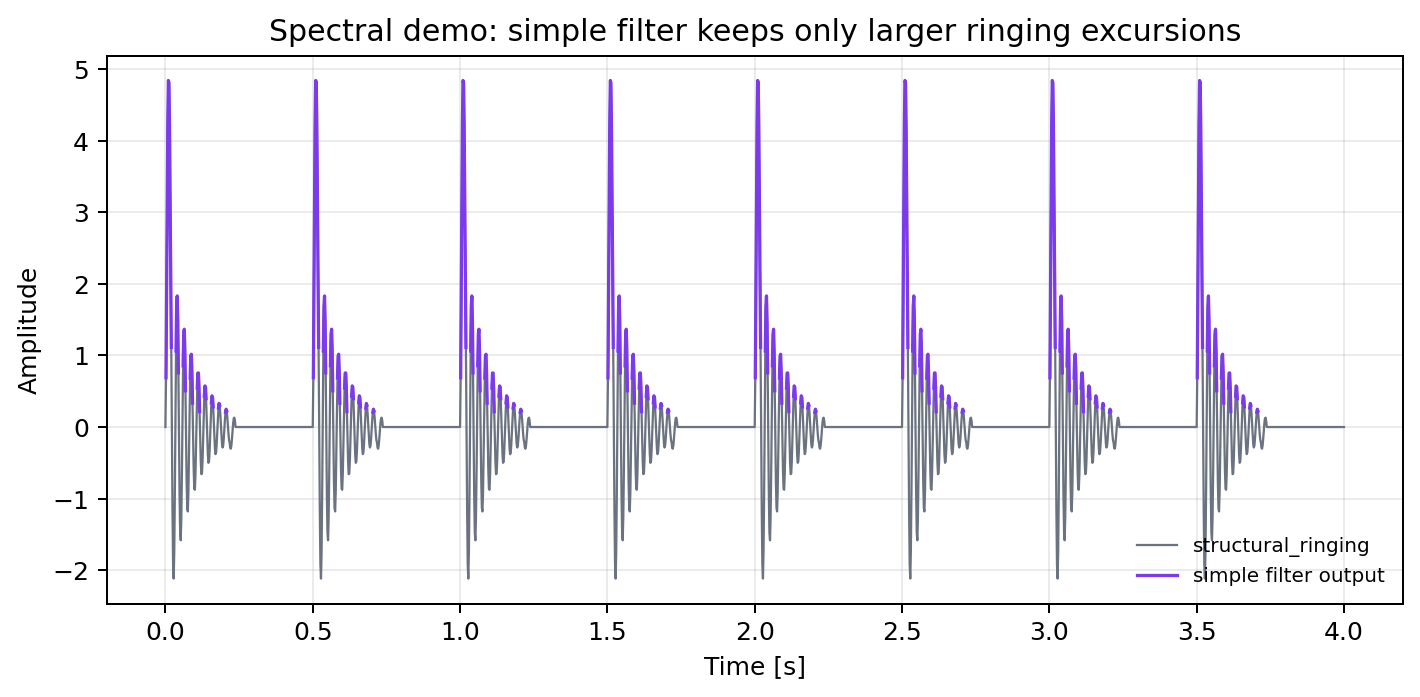
\includegraphics[width=0.9\linewidth]{simple_filter_mask_example.png}
    \caption{Simple filtering on the built-in spectral demo. The example keeps only larger values of the known \texttt{structural\_ringing} component. The row count stays unchanged; only the output column is masked.}
\end{figure}

\section{Smoothing Filters}

\subsection{Moving Average}

The moving average is a local low-pass smoother. For an odd window width $W = 2m + 1$,

\[
y[n] = \frac{1}{W} \sum_{k=-m}^{m} x[n+k].
\]

In EvalData this is implemented as a centered rolling mean.

Use it when the signal is noisy but the underlying variation is slower than the sample-to-sample fluctuations.

\subsection{Median Filter}

The median filter replaces each point by the median of its local neighborhood:

\[
y[n] = \mathrm{median}\{x[n-m], \dots, x[n+m]\}.
\]

This is less sensitive to isolated spikes than a moving average.

Use it when you want smoothing that is more resistant to outliers.

\subsection{Exponential Smoothing}

Exponential smoothing is recursive:

\[
y[n] = \alpha x[n] + (1-\alpha) y[n-1], \qquad 0 < \alpha \le 1.
\]

Smaller $\alpha$ produces heavier smoothing and more lag.

\begin{figure}[ht]
    \centering
    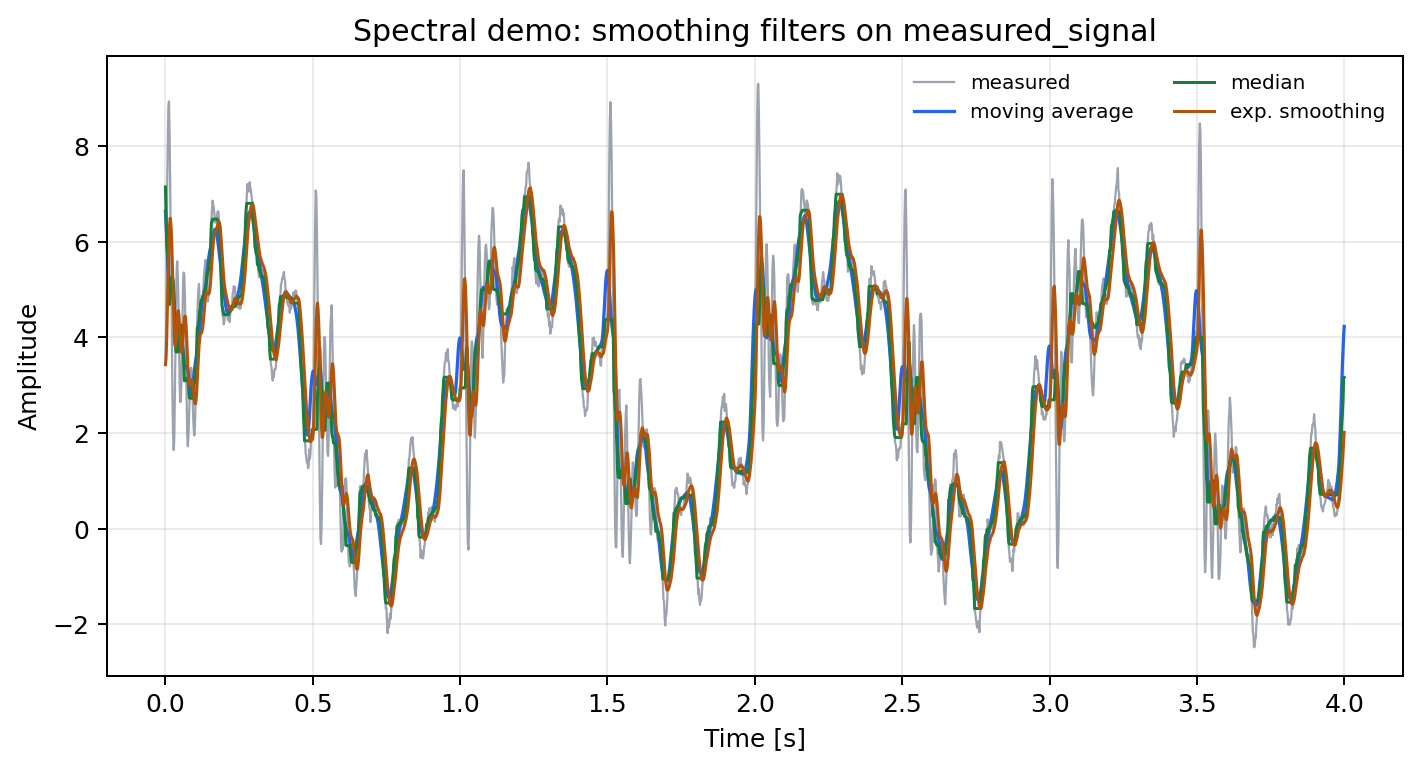
\includegraphics[width=0.9\linewidth]{filter_smoothing_comparison.png}
    \caption{Three smoothing filters applied to the deterministic \texttt{measured\_signal} channel from the built-in spectral demo. The comparison is reproducible because the demo signal is fixed.}
\end{figure}

\section{High-Pass Filtering}

The current high-pass option in EvalData is implemented as

\[
y[n] = x[n] - \mathrm{LP}_{W}\{x[n]\},
\]

where $\mathrm{LP}_{W}$ is the moving-average trend computed with the chosen window size.

This is a pragmatic trend-removal method rather than a full designed digital high-pass filter with a specified frequency response.

Use it when you want to suppress slow drift and emphasize faster variations.

\begin{figure}[ht]
    \centering
    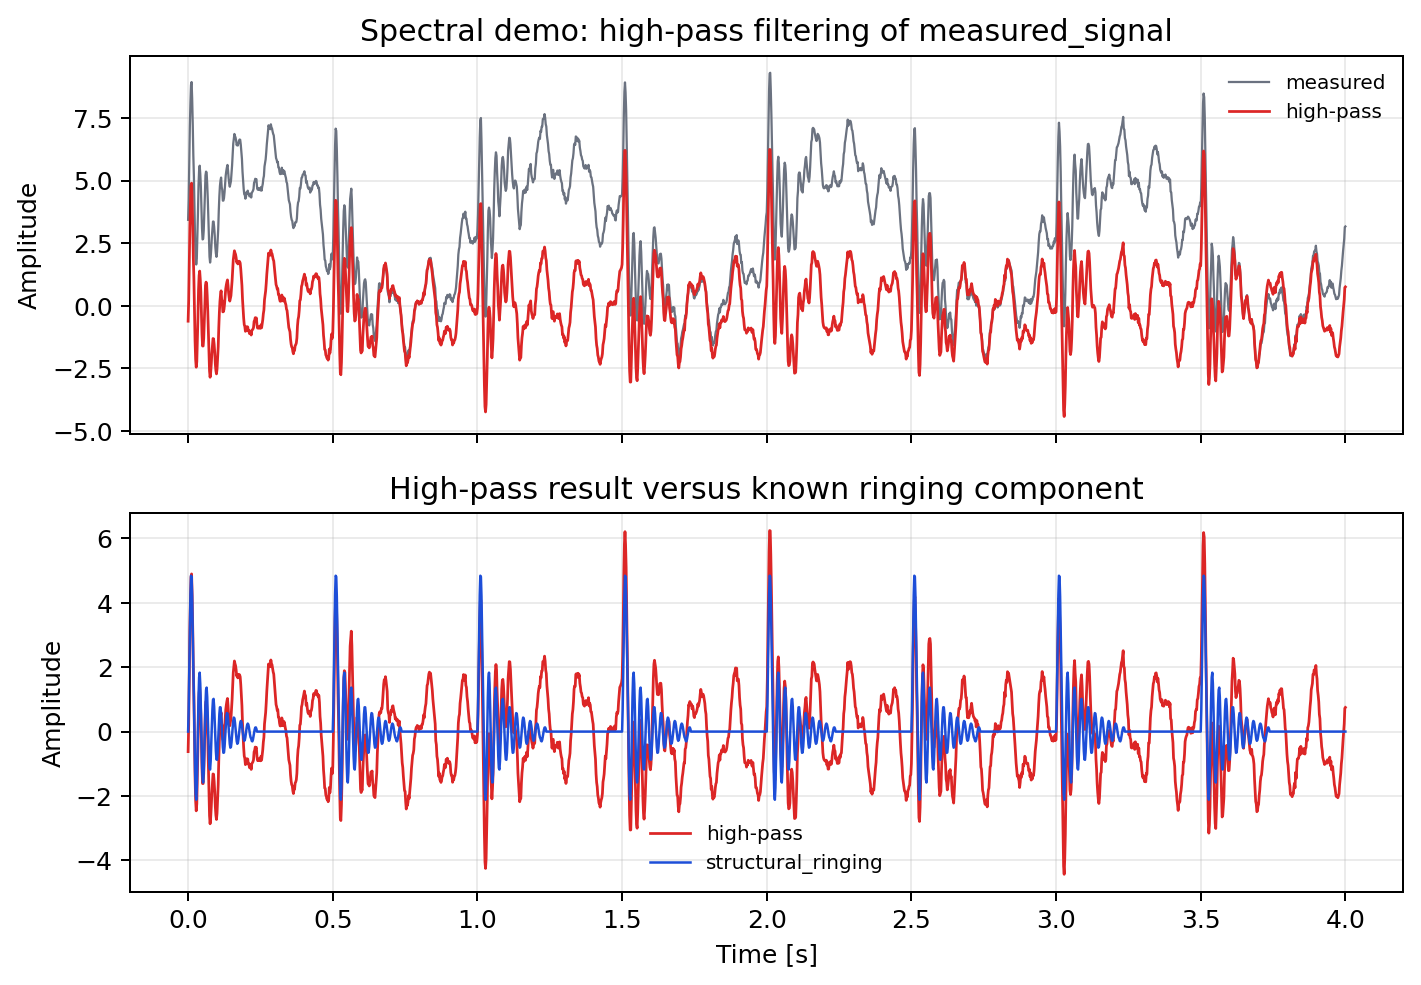
\includegraphics[width=0.9\linewidth]{high_pass_ringing_comparison.png}
    \caption{High-pass filtering on the built-in spectral demo. The lower panel compares the high-pass result against the known \texttt{structural\_ringing} component included in the synthetic dataset.}
\end{figure}

\section{Butterworth Filters}

EvalData also exposes zero-phase Butterworth filters for lowpass, highpass, and bandpass operation. These are designed digital IIR filters with a maximally flat magnitude response in the passband.

\subsection{Butterworth Transfer Function}

The squared magnitude response of an $N$-th order Butterworth lowpass filter with cutoff frequency $f_c$ is

\[
|H(f)|^2 = \frac{1}{1 + \left(\frac{f}{f_c}\right)^{2N}}.
\]

At the cutoff frequency $f = f_c$ the gain is $-3$\,dB regardless of filter order. Higher order $N$ gives a steeper roll-off.

For a digital implementation, the analog prototype is mapped to a discrete-time filter using the bilinear transform. The cutoff frequency must be normalized to the Nyquist frequency $f_{\mathrm{Ny}} = f_s / 2$:

\[
W_n = \frac{f_c}{f_{\mathrm{Ny}}}, \qquad 0 < W_n < 1.
\]

\subsection{Lowpass}

A Butterworth lowpass filter passes frequencies below $f_c$ and attenuates frequencies above it. It is used to suppress high-frequency noise while preserving slower signal content.

\subsection{Highpass}

A Butterworth highpass filter passes frequencies above $f_c$ and attenuates frequencies below it. It is used to remove slow trends or DC offsets while preserving faster oscillations.

\subsection{Bandpass}

A Butterworth bandpass filter passes frequencies in the range $[f_{\mathrm{low}}, f_{\mathrm{high}}]$ and attenuates content outside that band. Two normalized cutoff frequencies are required:

\[
W_{n,1} = \frac{f_{\mathrm{low}}}{f_{\mathrm{Ny}}}, \qquad W_{n,2} = \frac{f_{\mathrm{high}}}{f_{\mathrm{Ny}}}, \qquad 0 < W_{n,1} < W_{n,2} < 1.
\]

\subsection{Zero-Phase Implementation}

All three Butterworth filter types use zero-phase filtering via \texttt{sosfiltfilt}. The filter is applied forward and then backward, which squares the magnitude response and eliminates phase distortion:

\[
y[n] = \mathrm{sosfiltfilt}(\mathrm{SOS}, x[n]),
\]

where $\mathrm{SOS}$ is the second-order sections representation produced by \texttt{scipy.signal.butter}. Because the filter is applied twice, the effective order is doubled: an $N$-th order design yields a $2N$-th order zero-phase response.

\subsection{Parameters}

\begin{itemize}
    \item \textbf{Filter order} $N$: controls roll-off steepness. EvalData clamps to $1 \le N \le 10$.
    \item \textbf{Cutoff frequency} $f_c$ (Hz): the $-3$\,dB point. Must satisfy $0 < f_c < f_{\mathrm{Ny}}$. Bandpass requires two values.
    \item \textbf{Sample spacing} $\Delta t$ (s): the uniform time step between samples. Required so that $f_s = 1/\Delta t$ is known.
    \item The signal must contain at least $3N + 1$ valid samples for stable filtering.
\end{itemize}

\section{What the Demo Shows}

The spectral reference demo contains several ingredients on purpose:

\begin{itemize}
    \item slow drift near 0.15 Hz,
    \item clean periodic content near 1.0 Hz, 7.5 Hz, and 18.0 Hz,
    \item repeated impacts,
    \item decaying structural ringing near 42 Hz,
    \item seeded broadband noise.
\end{itemize}

That makes it a useful control case for filtering documentation:

\begin{itemize}
    \item smoothing can reduce the seeded noise,
    \item high-pass filtering can suppress the slow drift,
    \item simple filtering can isolate larger ringing excursions.
\end{itemize}

\section{Practical Interpretation Limits}

These methods are useful, but they have limits:

\begin{itemize}
    \item stronger smoothing also blurs short events,
    \item median and moving-average filters do not preserve the same features equally well,
    \item exponential smoothing introduces lag,
    \item the moving-average high-pass option should not be described as a precise frequency-domain filter design,
    \item Butterworth filters require correct sample spacing; wrong spacing shifts all frequency interpretations,
    \item Butterworth bandpass requires two well-separated cutoff frequencies below the Nyquist limit,
    \item zero-phase filtering cannot be applied causally in real-time applications,
    \item a masked simple-filter output is not the same thing as row-wise trimming.
\end{itemize}

Those distinctions matter because the user-visible controls are operationally simple, but their outputs answer different questions.

\section{Conclusion}

EvalData's current filtering tools span two levels: lightweight smoothing and trend-removal tools (moving average, median, exponential smoothing, moving-average high-pass) and designed digital filters (Butterworth lowpass, highpass, bandpass with zero-phase application). Simple filtering remains a masking tool. The built-in spectral demo gives a reproducible reference case for showing the difference between those behaviors without relying on private measurement data.

\begin{thebibliography}{9}

\bibitem{oppenheim2010}
A.~V.~Oppenheim and R.~W.~Schafer,
\emph{Discrete-Time Signal Processing}, 3rd~ed.
Upper Saddle River, NJ: Pearson, 2010.

\bibitem{smith1997}
S.~W.~Smith,
\emph{The Scientist and Engineer's Guide to Digital Signal Processing}.
San Diego, CA: California Technical Publishing, 1997.
Available: \url{https://www.dspguide.com/}

\bibitem{butterworth1930}
S.~Butterworth,
``On the theory of filter amplifiers,''
\emph{Wireless Engineer}, vol.~7, no.~6, pp.~536--541, 1930.

\bibitem{parks1987}
T.~W.~Parks and C.~S.~Burrus,
\emph{Digital Filter Design}.
New York, NY: Wiley, 1987.

\bibitem{gustafsson1996}
F.~Gustafsson,
``Determining the initial states in forward-backward filtering,''
\emph{IEEE Trans.\ Signal Processing}, vol.~44, no.~4, pp.~988--992, 1996.

\end{thebibliography}

\end{document}